\section{Оптимальные результаты для игрока С}

Теперь рассмотрим игру с точки зрения игрока С. Для каждой пары параметров $(\hat\mu, \hat\lambda)$ найдём
множество соответсвующих оптимальных пар $(p^*(\hat\mu, \hat\lambda), q^*(\hat\mu, \hat\lambda))$. Далее 
найдём значение свёртки для игрока С в этих точка:
$$
M(p^*,q^*,\hat\mu)=p^*\min{\{\frac{q^*}{\hat\mu};\frac{1-q^*}{2(1-\hat\mu)}\}} +
				   (1-p^*)\min\{\frac{q^*}{2\hat\mu};\frac{1-q^*}{1-\hat\mu}\}
$$
И изобразим множество значений функции в этих точках.
\vspace{5mm}
 
Рассмотрим все возможные сочетания значений для $p^{*}$ и $q^{*}$ в системах (7) и (8), что даст нам 6 следующих систем:
\vspace{5mm}

Напомню, что переменные имеют следующих области ограничений:
\[
p \in [0, 1],\quad q \in [0, 1],\quad
\mu \in [0, 1],\quad \lambda \in [0, 1]
\]
\circled{1}%---------------------------1------------------------
\[
\begin{cases}
p^{*}=0 \\
q^{*}=\frac{\mu}{2-\mu} \\
q^{*}>1-\lambda \\
p^{*}+\mu-1\geq 0 \\
\end{cases}
\quad\sim\quad
\begin{cases}
p^{*}=0 \\
q^{*}=\frac{\mu}{2-\mu} \\
\frac{\mu}{2-\mu}>1-\lambda \\
\mu\geq 1 \quad\Rightarrow\quad \mu=1 \\
\end{cases}
\quad\sim\quad
\begin{cases}
p^{*}=0 \\
q^{*}=1 \\
\lambda>0 \\
\mu=1
\end{cases}
\]
Значит при $\mu=1$, $\lambda\in(0,1]$ имеем следующие оптимальные пары
$\begin{cases}p^{*}=0 \\ q^{*}=1 \end{cases}$

\circled{2}%---------------------------2------------------------
\[
\begin{cases}
p^{*}=0 \\
q^{*}=\frac{2\mu}{1+\mu} \\
q^{*}>1-\lambda \\
p^{*}+\mu-1\leq 0 \\
\end{cases}
\quad\sim\quad
\begin{cases}
p^{*}=0 \\
q^{*}=\frac{2\mu}{1+\mu} \\
\frac{2\mu}{1+\mu}>1-\lambda \\
\mu \leq 1
\end{cases}
\quad\sim\quad
\begin{cases}
p^{*}=0 \\
q^{*}=\frac{2\mu}{1+\mu} \\
\lambda>\frac{1-\mu}{1+\mu} \\
\mu \leq 1
\end{cases}
\]
Значит при $\mu \in [0, 1]$, $\lambda \in (\frac{1-\mu}{1+\mu}, 1]$ имеем следующие оптимальные пары
$\begin{cases}p^{*}=0 \\ q^{*}=\frac{2\mu}{1+\mu} \end{cases}$



\circled{3}%---------------------------3------------------------
\[
\begin{cases}
p^{*}=1 \\
q^{*}=\frac{\mu}{2-\mu} \\
q^{*}<1-\lambda \\
p^{*}+\mu-1\geq 0 \\
\end{cases}
\quad\sim\quad
\begin{cases}
p^{*}=1 \\
q^{*}=\frac{\mu}{2-\mu} \\
\frac{\mu}{2-\mu}<1-\lambda \\
\mu \geq 0
\end{cases}
\quad\sim\quad
\begin{cases}
p^{*}=1 \\
q^{*}=\frac{\mu}{2-\mu} \\
\lambda<2\frac{1-\mu}{2-\mu} \\
\mu \geq 0
\end{cases}
\]
Значит при $\mu \in [0, 1]$, $\lambda \in [0, 2\frac{1-\mu}{2-\mu})$ имеем следующие оптимальные пары
$\begin{cases}p^{*}=1 \\ q^{*}=\frac{\mu}{2-\mu} \end{cases}$


\circled{4}%---------------------------4------------------------
\[
\begin{cases}
p^{*}=1 \\
q^{*}=\frac{2\mu}{1+\mu} \\
q^{*}<1-\lambda \\
p^{*}+\mu-1 \leq 0 \\
\end{cases}
\quad\sim\quad
\begin{cases}
p^{*}=1 \\
q^{*}=\frac{2\mu}{1+\mu} \\
\frac{2\mu}{1+\mu}<1-\lambda \\
\mu \leq 0 \quad\Rightarrow\quad \mu=0 \\
\end{cases}
\quad\sim\quad
\begin{cases}
p^{*}=1 \\
q^{*}=0 \\
\lambda<1 \\
\mu=0
\end{cases}
\]
Значит при $\mu=0$, $\lambda \in [0, 1)$ имеем следующие оптимальные пары
$\begin{cases}p^{*}=1 \\ q^{*}=0 \end{cases}$


\circled{5} %---------------------------5------------------------
\[
\begin{cases}
p^{*} \in [0, 1] \\
q^{*}=\frac{\mu}{2-\mu} \\
q^{*}=1-\lambda \\
p^{*}+\mu-1 \geq 0 \\
\end{cases}
\quad\sim\quad
\begin{cases}
p^{*} \in [0, 1] \\
q^{*}=\frac{\mu}{2-\mu} \\
\frac{\mu}{2-\mu}=1-\lambda \\
p^* \geq 1-\mu \\
\end{cases}
\quad\sim\quad
\begin{cases}
p^* \in [1-\mu, 1] \\
q^{*}=\frac{\mu}{2-\mu} \\
\lambda=2\frac{1-\mu}{2-\mu} \\
\end{cases}
\]
Значит при $\lambda=2\frac{1-\mu}{2-\mu}$, $\mu \in [0, 1]$ имеем следующие оптимальные пары
$\begin{cases}p^{*} \in [1-\mu, 1] \\ q^{*}=\frac{\mu}{2-\mu} \end{cases}$


\circled{6}%---------------------------6------------------------
\[
\begin{cases}
p^{*} \in [0, 1] \\
q^{*}=\frac{2\mu}{1+\mu} \\
q^{*}=1-\lambda \\
p^{*}+\mu-1 \leq 0 \\
\end{cases}
\quad\sim\quad
\begin{cases}
p^{*} \in [0, 1] \\
q^{*}=\frac{2\mu}{1+\mu} \\
\frac{2\mu}{1+\mu}=1-\lambda \\
p^{*} \leq 1 - \mu 
\end{cases}
\quad\sim\quad
\begin{cases}
p^{*} \in [0, 1-\mu] \\
q^{*}=\frac{2\mu}{1+\mu} \\
\lambda = \frac{1-\mu}{1+\mu} \\
\end{cases}
\]
Значит при $\mu \in [0, 1]$, $\lambda = \frac{1-\mu}{1+\mu} $ имеем следующие оптимальные пары
$\begin{cases}
p^{*} \in [0, 1-\mu] \\
q^{*}=\frac{2\mu}{1+\mu} \\
\end{cases}$
\vspace{10mm}

Теперь на квадрате $(p,q)\in[0, 1]^{2}$ рассмотрим все области, в которых множества оптимальных пар постоянны. И найдём множества значений функции 
\[
M(p,q,\mu)=p\min{\{\frac{q}{\mu};\frac{1-q}{2(1-\mu)}\}}+(1-p)\min\{\frac{q}{2\mu};\frac{1-q}{1-\mu}\}
\]
В этих областях

\begin{center}
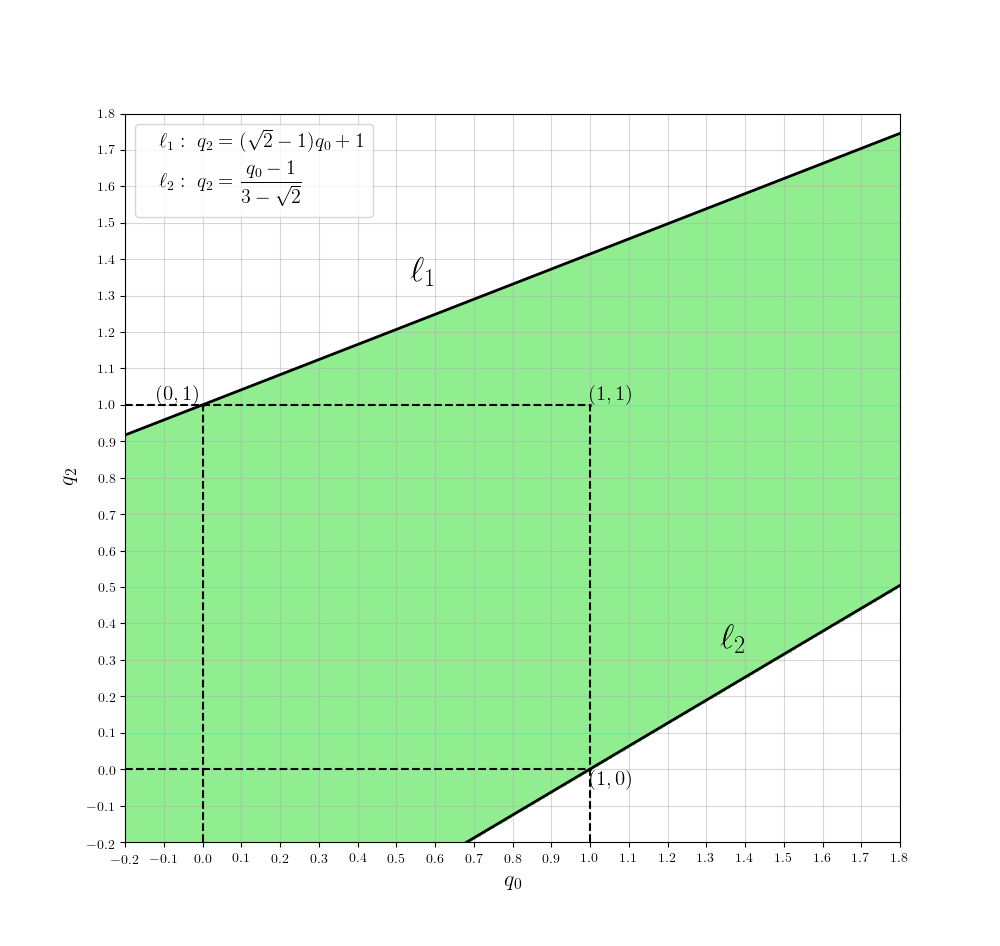
\includegraphics[scale=0.4]{graf_3_1}
\end{center}

1) $\mu=0$, $\lambda \in [0, 1)$: 
$\begin{cases}p^{*}=1 \\ q^{*}=0 \end{cases};
\begin{cases}p^{*}=1 \\ q^{*}=\frac{\mu}{2-\mu} 
= \{\mu=0\}=0 \end{cases} $ \hfill \break
Получаем множества оптимальных стратегий 
$(P^{*} \times Q^{*}) =(\{1\} \times \{0\})$, где $\times$ - это декартово произведение, тогда
$$M(1,0,0)=\frac{1}{2}$$


\begin{center}
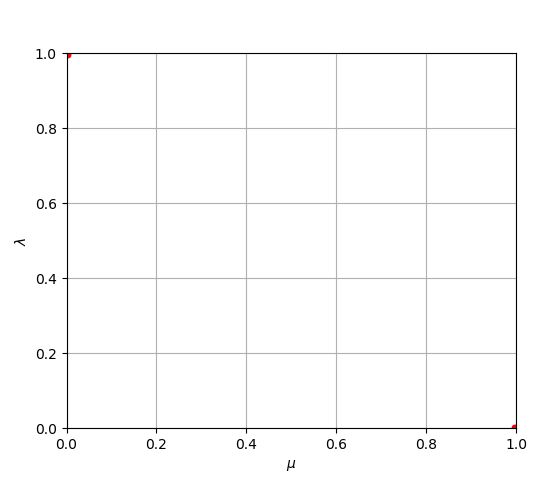
\includegraphics[scale=0.7]{graf_3_2}
\end{center}
2.1) $\mu=0$, $\lambda =1$: 
$\begin{cases}p^{*} \geq 1-\mu = \{\mu=0\}=1
\\ q^{*}=\frac{\mu}{2-\mu} = \{\mu=0\}=0
\end{cases}$;
$\begin{cases}p^{*} \leq 1-\mu = \{\mu=0\}=1\\\
q^{*}=\frac{2\mu}{1+\mu}= \{\mu=0\}=0 \end{cases}$
\hfill \break 
Получаем множества оптимальных стратегий 
$(P^{*} \times Q^{*}) =([0, 1] \times \{0\})$ тогда
$$M([0, 1],0,0)=[0.5,1]$$
%\vspace{5mm}

2.2) $\mu=1$, $\lambda=0$: 
$\begin{cases}p^{*} \geq 1-\mu = \{\mu=1\}=0
\\ q^{*}=\frac{\mu}{2-\mu} = \{\mu=1\}=1
\end{cases}$;
$\begin{cases}p^{*} \leq 1-\mu = \{\mu=1\}=0\\\
q^{*}=\frac{2\mu}{1+\mu}= \{\mu=1\}=1 \end{cases}$
\hfill \break 
Получаем множества оптимальных стратегий 
$(P^{*} \times Q^{*}) =([0, 1] \times \{1\})$ тогда
$$M([0, 1],1,1)=[0.5,1]$$
%\vspace{5mm}

\begin{center}
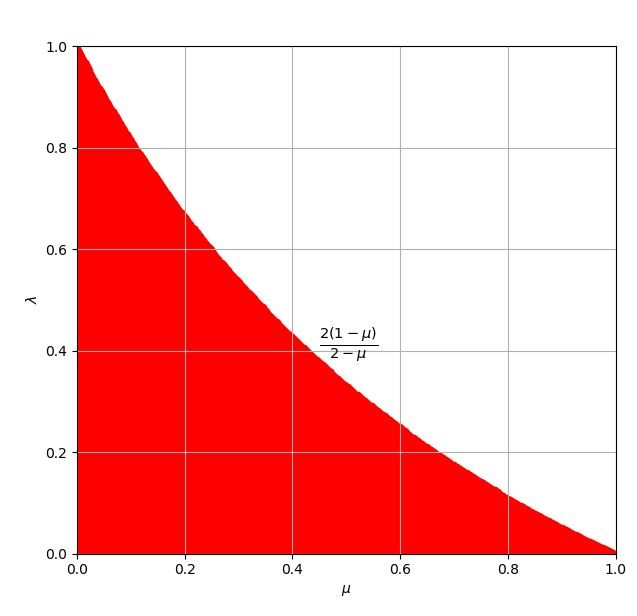
\includegraphics[scale=0.6]{graf_3_3}
\end{center}
3) $\mu \in (0,1)$, $\lambda\in(0,\frac{1-\mu}{1+\mu}]$: 
$\begin{cases}p^{*}=1 \\ q^{*}=\frac{\mu}{2-\mu} \end{cases}$
\hfill \break
Получаем множества оптимальных стратегий 
$(P^{*} \times Q^{*}) =(\{1\} \times \{\frac{\mu}{2-\mu}\})$ тогда
$$M(1,\frac{\mu}{2-\mu},\mu)=\min \big\{\frac{\mu}{2-\mu}; 
\frac{1-\frac{\mu}{2-\mu}}{2(1-\mu)}\big\}=\frac{1}{2-\mu}$$
%\vspace{5mm}

\begin{center}
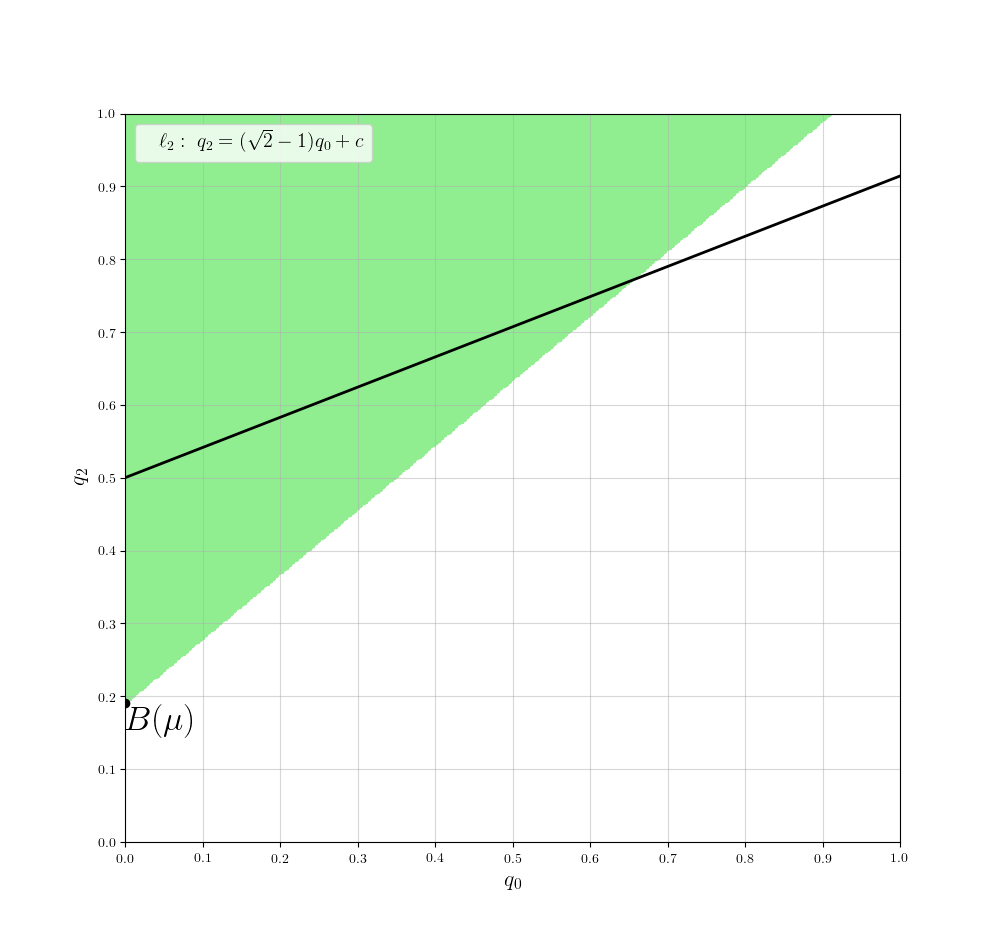
\includegraphics[scale=0.6]{graf_3_4}
\end{center}
4) $\mu \in (0,1)$, $\lambda=\frac{1-\mu}{1+\mu}$:
$\begin{cases}p^{*} \in [0, 1-\mu] \cup \{1\} \\
q^{*} = \frac{\mu}{2-\mu}
\end{cases}$
\hfill \break
4.1) Получаем множества оптимальных стратегий 
$(P^{*} \times Q^{*}) =(\{1\} \times \{\frac{\mu}{2-\mu}\})$ тогда
$$M(1,\frac{\mu}{2-\mu},\mu)=\frac{1}{2-\mu}$$

4.2) Получаем множества оптимальных стратегий 
$(P^{*} \times Q^{*}) =([0,1-\mu] \times \{\frac{2\mu}{1+\mu}\})$ тогда
$$M(p,\frac{2\mu}{1+\mu},\mu)=p\frac{1}{2(1+\mu)}+(1-p)\frac{1}{1+\mu}=\frac{2-p}{2(1+\mu)} \geq
\frac{2 - (1-\mu)}{2(1+\mu)}=\frac{1+\mu}{2(1+\mu)}=\frac{1}{2}$$
$$M(p,\frac{2\mu}{1+\mu},\mu) \leq \frac{1}{1+\mu} \Rightarrow M(p,\frac{2\mu}{1+\mu},\mu) = [0.5, \frac{1}{1+\mu}]$$

\begin{center}
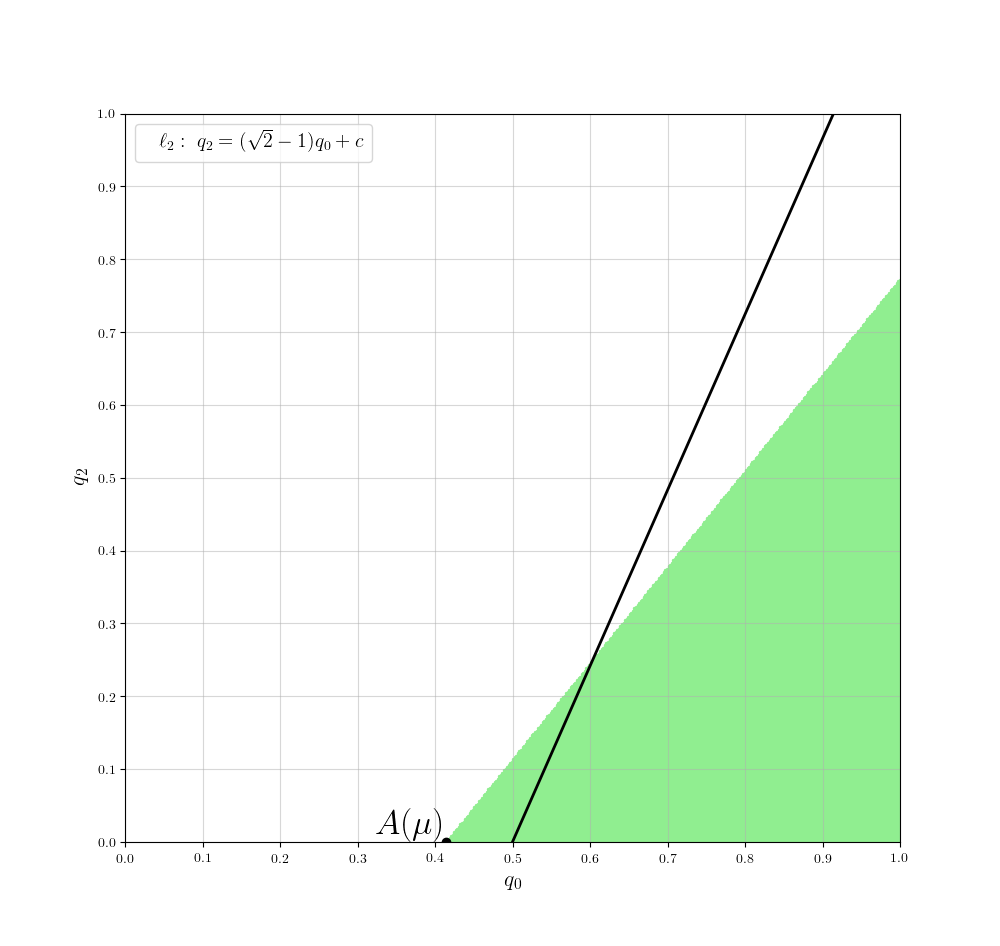
\includegraphics[scale=0.5]{graf_3_5}
\end{center}
5) $\mu \in [(, 1)$, $\lambda \in [0, 2\frac{1-\mu}{2-\mu}]\cap(\frac{1-\mu}{1+\mu}, 1]$: 
$\begin{cases}p^{*}=0 \\ q^{*}=\frac{2\mu}{1+\mu} \end{cases}$;
$\begin{cases}p^{*}=1 \\ q^{*}=\frac{\mu}{2-\mu} \end{cases}$
\hfill \break
5.1) Получаем множества оптимальных стратегий 
$(P^{*} \times Q^{*}) =(\{0\} \times \{\frac{2\mu}{1+\mu}\})$ тогда
$$M(0, \frac{2\mu}{1+\mu},\mu)=\frac{1}{1+\mu}$$
5.2) Получаем множества оптимальных стратегий 
$(P^{*} \times Q^{*}) =(\{1\}\times \{\frac{\mu}{2-\mu}\})$ тогда
$$M(1, \frac{\mu}{2-\mu},\mu)=\frac{1}{2-\mu}$$

\begin{center}
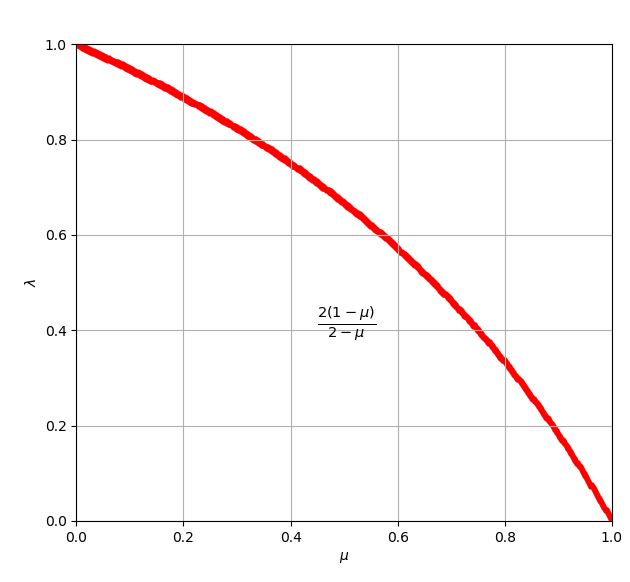
\includegraphics[scale=0.5]{graf_3_6}
\end{center}
6) $\mu \in (0, 1)$, $\lambda = 2\frac{1-\mu}{2-\mu}$: 
$\begin{cases}p^{*}=0 \\ q^{*}=\frac{2\mu}{1+\mu} \end{cases}$;
$\begin{cases}p^{*} \in [0,1-\mu] \\ q^{*}=\frac{\mu}{2-\mu} \end{cases}$
\hfill \break
6.1) Получаем множества оптимальных стратегий 
$(P^{*} \times Q^{*}) =(\{0\} \times \{\frac{2\mu}{1+\mu}\})$ тогда
$$M(0, \frac{2\mu}{1+\mu}, \mu)=\frac{1}{1+\mu}$$
6.2) Получаем множествo оптимальных стратегий 
$(P^{*}\times Q^{*}) =([1-\mu,1] \times \{\frac{\mu}{2-\mu}\})$ тогда
$$M(p,\frac{\mu}{2-\mu},\mu)=p\frac{1}{2-\mu}+(1-p)\frac{1}{2(2-\mu)}=\frac{1+p}{2(2-\mu)} \geq \frac{2-\mu}{2(2-\mu)}=\frac{1}{2}$$
$$M(p,\frac{\mu}{2-\mu},\mu) \leq \frac{1}{2-\mu} \Rightarrow M(p,\frac{\mu}{2-\mu},\mu) = [0.5, \frac{1}{2-\mu}]$$


\begin{center}
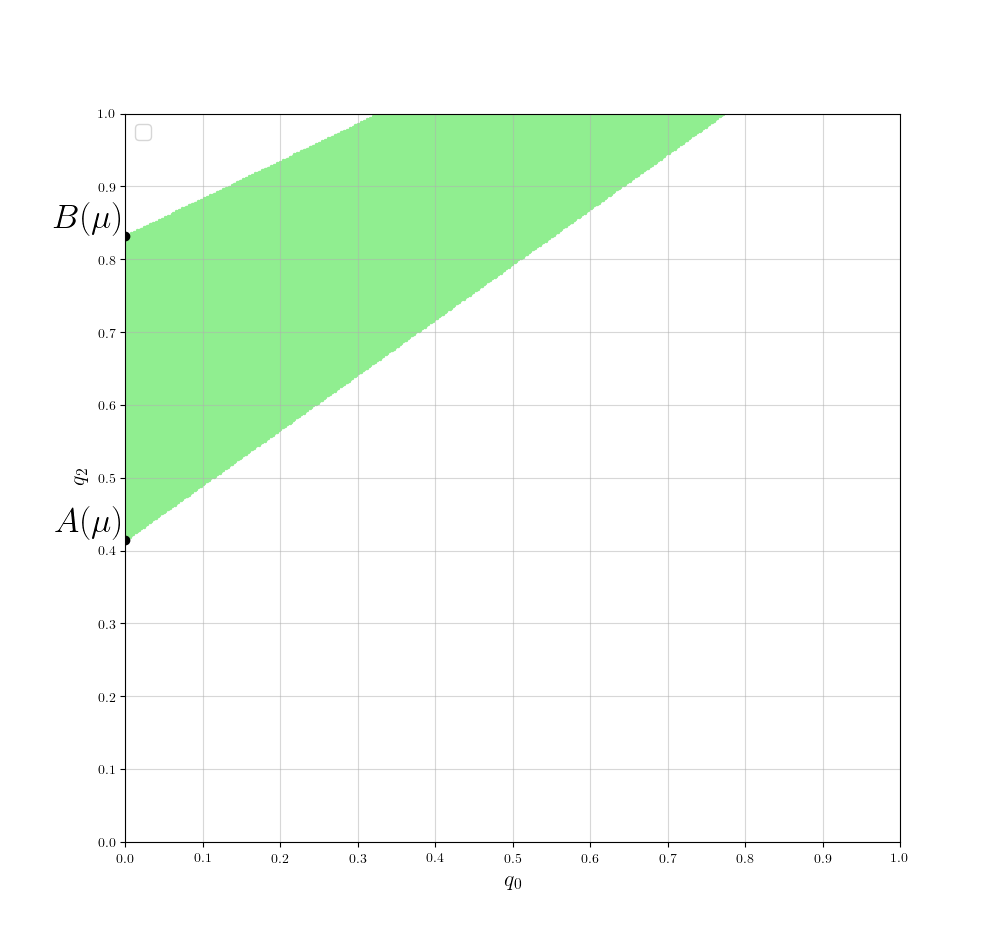
\includegraphics[scale=0.5]{graf_3_7}
\end{center}
7) $\mu \in (0, 1), \lambda \in (2\frac{1-\mu}{2-\mu}, 1]$: 
$\begin{cases}p^{*} =0 \\ q^{*}=\frac{2\mu}{1+\mu} \end{cases}$
\hfill \break
Получаем множества оптимальных стратегий 
$(P^{*} \times Q^{*}) =(\{0\} \times \{\frac{2\mu}{1+\mu}\})$ тогда
$$M(0, \frac{2\mu}{1+\mu}, \mu)=\min \big\{\frac{1}{\mu}\frac{2\mu}{1+\mu}; 
\frac{1-\frac{2\mu}{1+\mu}}{1-\mu}\big\}=\frac{1}{1+\mu}$$

\begin{center}
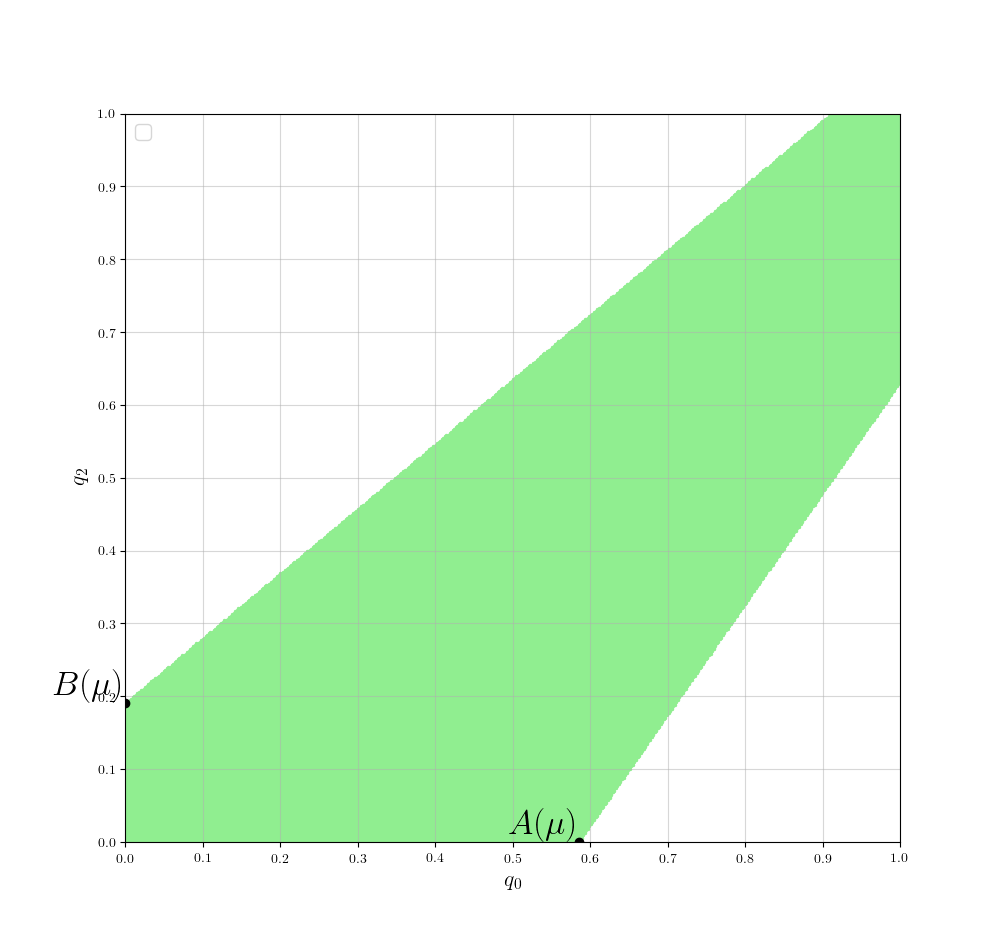
\includegraphics[scale=0.5]{graf_3_8}
\end{center}
8) $\mu = 1$, $\lambda \in (0, 1] $: 
$\begin{cases}
p^{*}=0 \\
q^{*}=1 \\
\end{cases}$;
$\begin{cases}
p^{*}=0 \\
q^{*}=\frac{2\mu}{1+\mu}=\{\mu=1\}=1 \\
\end{cases}$
\hfill \break
Получаем множества оптимальных стратегий 
$(P^{*} \times Q^{*}) =(\{0\} \times \{1\})$ тогда
$$M(0, 1, 1)=\frac{1}{2}$$
\vspace{40mm}

Теперь на квадрате $(\mu,\lambda)\in[0, 1]^{2}$ мы рассмотрели все точки и для каждой нашли оптимальные пары $p^{*}(\mu, \lambda)$
и $q^{*}(\mu, \lambda)$ и соответсвующие значения функции $M(p^{*}(\mu, \lambda),q^{*}(\mu, \lambda),\mu)$. Далее на квадрате
$[0, 1]^{2}$ изобразим все точки, которые принимает вектор $(\mu M(p^{*},q^{*},\mu), (1-\mu) M(p^{*},q^{*},\mu))$ при
$(\mu, \lambda)\in[0, 1]^{2}$

\begin{center}
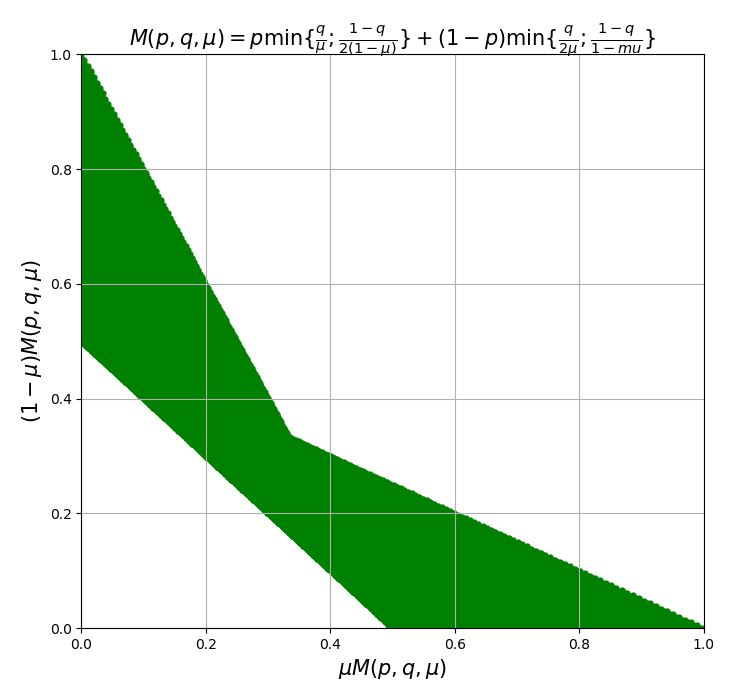
\includegraphics[scale=0.6]{graf_4}
\end{center}

Поясним график: \\
нижняя огибающая в координатах $X,Y$: $y=\frac{1}{2}-x$, \\
верхняя огибающая в координатах $X,Y$: $y=
\begin{cases}
1-2x, & x \in [0, \frac{1}{3}) \\
\frac{1-x}{2}, & x \in [\frac{1}{3}, 1]
\end{cases}.
$
